\documentclass[floatfix,nofootinbib,superscriptaddress,fleqn]{revtex4-2} 
%\documentclass[aps,epsfig,tightlines,fleqn]{revtex4}
\usepackage[utf]{kotex}
\usepackage[HWP]{dhucs-interword}
\usepackage[dvips]{color}
\usepackage{graphicx}
\usepackage{bm}
%\usepackage{fancyhdr}
%\usepackage{dcolumn}
\usepackage{defcolor}
\usepackage{amsmath}
\usepackage{amsfonts}
\usepackage{amssymb}
\usepackage{amscd}
\usepackage{amsthm}
\usepackage[utf8]{inputenc}
 \usepackage{setspace}
 \usepackage{tikz}
%\pagestyle{fancy}

\begin{document}

\title{\Large 2022년 1학기 물리학 I: Quiz 13}
\author{김현철} 
\author{Lee Hui-Jae} 
\email{hchkim@inha.ac.kr}
\email{hjlee6674@inha.edu}
\affiliation{Hadron Theory Group, Department of Physics,
Inha University, Incheon 22212, Republic of Korea }
\date{Spring semester, 2022}


\vspace{1.cm}

\maketitle


\noindent {\bf 문제 1. (20 pt)}
발사체를 지구 탈출속력의 1/2배의 속력으로 지표면에서 연직 위로 발사
한다. 지구의 반지름이 $R_{\oplus}$라면 발사체가 도달하는 최고높이는
얼마인가? 

\noindent {\bf 풀이 : }
우선 지구 탈출속력을 구해보자. 탈출속력을 $v_e$, 지구의 질량을 $M_\oplus$, 
발사체의 질량을 $m$이라고 하면 발사체가 지구 표면에 있을 때의 역학적 에너지 $E$는,
\begin{align}
    E = -\frac{GM_\oplus m}{R_\oplus} + \frac{1}{2}mv^2_e=0.
\end{align}
따라서 탈출속력 $v_e$는 다음과 같다.
\begin{align}
    v_e = \sqrt{\frac{2GM_\oplus}{R_\oplus}}.
\end{align}
발사체가 탈출속력의 1/2배의 속력으로 지구를 떠난다면 발사체가 지구 표면에 있을 때의 
역학적 에너지 $E_1$는,
\begin{align}
    E_1 = -\frac{GM_\oplus m}{R_\oplus} + \frac{1}{8}mv_e^2
    =-\frac{3GM_\oplus m}{4R_\oplus}.
\end{align}
발사체가 최대높이 $h$에 있을 때 발사체의 속력은 0이다. 따라서 역학적 에너지 $E_2$는,
\begin{align}
    E_2 = -\frac{GM_\oplus m}{R+h}.
\end{align}
에너지 보존 법칙에 의해,
\begin{align}\label{eq:1-2}
    E_1 =E_2,\,\,\,
    -\frac{3GM_\oplus m}{4R_\oplus}=-\frac{GM_\oplus m}{R+h}.
\end{align}
그러므로 최대높이 $h$는 다음과 같다.
\begin{align}
    h = \frac{1}{3}R_\oplus.
\end{align}
발사체의 최대 높이 $h$가 지구의 반지름 $R_\oplus$에 비해 무시할 수 있을 만큼 
작다고 가정하여 근사를 취해보자. 식~\eqref{eq:1-2}로 부터,
\begin{align}\label{eq:1-3}
    \frac{3}{4R_\oplus}=\frac{1}{R_\oplus+h}
    =\frac{1}{R_\oplus}\left(\frac{1}{1+h/R_\oplus}\right).
\end{align}
$\frac{1}{1+h/R}$을 급수로 전개하면,
\begin{align}
    \frac{1}{1+h/R_\oplus} \approx
    1-\frac{h}{R_\oplus}+\left(\frac{h}{R_\oplus}\right)^2
    -\left(\frac{h}{R_\oplus}\right)^3
    +\left(\frac{h}{R_\oplus}\right)^4-\cdots.
\end{align}
$h/R_\oplus$에 대한 1차항만을 고려하였을 때 $h$는,
\begin{align}
    \frac{3}{4}=1-\frac{h}{R_\oplus},\,\,\,
    h = \frac{1}{4}R_\oplus.
\end{align}
$\frac{1}{3}R_\oplus$보다 작다.
2차항까지 고려한다면,
\begin{align}
    \frac{3}{4}=1-\frac{h}{R_\oplus}
    +\left(\frac{h}{R_\oplus}\right)^2,\,\,\,
    h = \frac{1}{2}R_\oplus.
\end{align}
이번에는 $\frac{1}{3}R_\oplus$보다 큰 값이 나온다.
3차항까지 고려한다면,
\begin{align}
    \frac{3}{4}=1-\frac{h}{R_\oplus}
    +\left(\frac{h}{R_\oplus}\right)^2
    -\left(\frac{h}{R_\oplus}\right)^3 ,\,\,\,
    h \approx 0.31945 R_\oplus
\end{align}
다시 이번에는 $\frac{1}{3}R_\oplus$보다 작다. 항을 계속 추가하여 고려하면
$h$는 $\frac{1}{3}R_\oplus$보다 커졌다 작아지면서 수렴한다. FIG.~\ref{fig:1}은 
1차항 부터 10차항 까지 고려하였을 때 $h$와 $R_\oplus$의 비율을 나타낸 것이다.
항을 더 많이 고려할 수록 $\frac{1}{3}$에 진동하며 수렴하는 형태를 볼 수 있다.
\begin{figure}[htp]
    \centering
  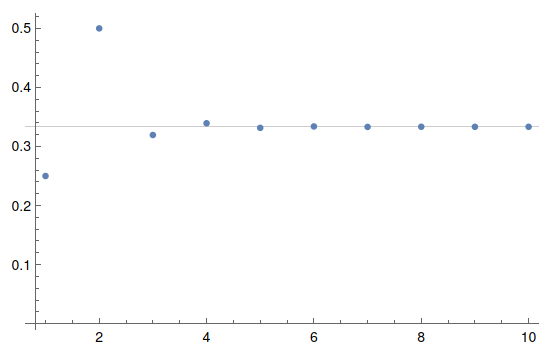
\includegraphics[scale=0.5]{pic_1-1.png}
    \caption{$h$와 $R_\oplus$의 비율}
    \label{fig:1}
  \end{figure}
\vspace{1.cm}

\noindent {\bf 문제 2. (40 pt)}
그림~\ref{fig:2}는 반지름이 $R=4.00$ cm인 납덩어리 공 내부에 공 모양의
공동이다. 공동의 표면은 안으로는 공의 중심을 지나고 밖으로는 공의
표면에 접한다. 공동을 만들기 전에 납덩어리 공의 질량은 $M=2.95$
kg이었다. 질량이 $m=0.431$ kg인 작은 공이 납덩어리의 중심에서 $d=9.00$
cm만큼 떨어져 있다. 두 공의 중심선이 공동의 중심을 지날 때 $m$에
미치는 중력을 구하여라.
\begin{figure}[htp]
  \centering
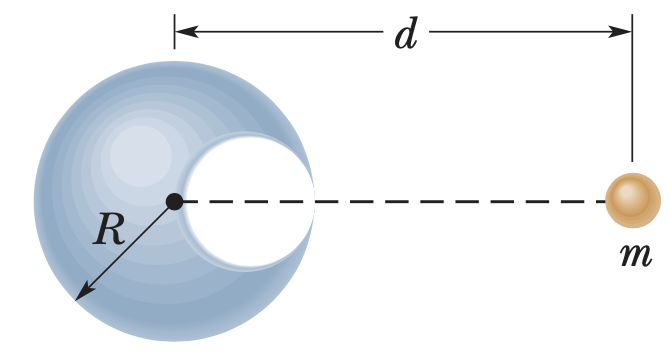
\includegraphics[scale=0.5]{Qfig13-1-20220425.png}
  \caption{문제 2}
  \label{fig:2}
\end{figure}

\noindent {\bf 풀이 : }
중첩 원리에 의해 물체 $m$에 작용하는 중력의 크기는 속이 찼을 때 
작용하는 중력에 공동 만큼의 물체에 의한 중력을 뺀 값과 같다.
물체 $M$의 밀도를 $\rho$라고 하면,
\begin{align}
    M = \frac{4}{3}R^3\rho ,\,\,\,\rho = \frac{3M}{4R^3}.
\end{align}
공동 만큼의 물체의 질량을 $M^\prime$이라고 하면,
\begin{align}
    M^\prime = \frac{4}{3}{\left(\frac{1}{2}R\right)}^3\rho=\frac{1}{8}M.
\end{align}
속이 찼을 때 중력을 $F_1$라고 하자. $F_1$은,
\begin{align}
    F_1 = \frac{GMm}{d^2}
\end{align}
공동 만큼의 중력을 $F_2$라고 하면 $F_2$는,
\begin{align}
    F_2 = \frac{GM^\prime m}{(d-\frac{1}{2}R)^2}=\frac{GMm}
    {2(2d-R)^2}.
\end{align}
위에서 말했듯이 실제 중력 $F$은 속이 찼을 때의 중력 $F_1$에 공동 만큼의 물체에 의한 중력 $F_2$를
뺀 값과 같다.
\begin{align}
    F= F_1 - F_2.
\end{align}
따라서,
\begin{align}
    F = GMm\left(\frac{1}{d^2}-\frac{1}{2(2d-R)^2}\right).
\end{align}
 G = $6.67430\times 10^{-11}\,\mathrm{N\cdot m^2/kg^2}$ 이므로 수치들을 모두 대입하고 계산해보자.
\begin{align}
    \begin{split}
        F &= \left(6.67430\times 10^{-11}\,\mathrm{N\cdot m^2/kg^2}\right)
        (2.95\,\mathrm{kg})(0.431\,\mathrm{kg})
        \left(\frac{1}{(9.00\,\mathrm{cm})^2}
        -\frac{1}{2(2(9.00\,\mathrm{cm})-(4.00\,\mathrm{cm}))^2}\right) \\
        &=  8.31\times 10^{-9}\,\mathrm{N}.  
    \end{split}
\end{align}
물체 $m$에 미치는 중력은 $8.31\times 10^{-9}\,\mathrm{N}$이다.

\vspace{1.cm}

\noindent {\bf 문제 3. (40pt)}
두 중성자별이 $1.0\times 10^{10}$ m 떨어져 있다. 각각의 질량은
$1.0\times 10^{30} $ kg이고, 반지름은 $1.0\times 10^5$ m이다. 두 별은
처음에 서로에 대해 정지해 있었다.
\begin{itemize}
\item[(가)] 두 별 사이의 거리가 처음의 반으로 줄어들 때 속력은
  얼마인가?
\item[(나)] 충돌하기 직전의 속력은 얼마인가?  
\end{itemize}

\noindent {\bf 풀이 : }
\begin{itemize}
  \item[(가)]
 중성자별 질량을 $m$, 반지름을 $r$, 
별이 서로 떨어진 거리를 $d$라 하자. 
계가 가진 처음 역학적 에너지를 $E_1$라고 하면,
\begin{align}
    E_1 = -\frac{Gm^2}{d}.
\end{align}
거리가 처음의 반이 되었을 때 계의 역학적 에너지는 다음과 같다.
\begin{align}
    E_2 = -\frac{2Gm^2}{d}+ \frac{1}{2}mv^2+\frac{1}{2}mv^2
    =-\frac{2Gm^2}{d}+ mv^2.
\end{align}
에너지 보존 법칙에 계의 역학적 에너지는 보존되므로,
\begin{align}
    E_1=E_2,\,\,\,-\frac{Gm^2}{d}=-\frac{2Gm^2}{d}+ mv^2.
\end{align}
속력 $v_2$에 대해 정리하여 속력 $v_2$를 구할 수 있다.
\begin{align}
    \begin{split}
        v_2 &= \sqrt{\frac{Gm}{d}} 
        =\sqrt{\frac{(6.67430\times 10^{-11}\,\mathrm{N\cdot m^2/kg^2})
        (1.0\times 10^{30}\,\mathrm{kg})}{(1.0\times 10^{10}\,\mathrm{m})}} \\
        &=8.2\times 10^4\mathrm{m/s}.
    \end{split}
\end{align}
각 별의 속력은 $8.2\times 10^4\mathrm{m/s}$이다. 혹은, $10^{10}\sqrt{G}$이다.
  \item[(나)] 
  충돌 직전이면 두 별 사이 거리가 $2r$인 상태이다. 이 때 별의 속력을 $v_f$라 하면 
계의 역학적 에너지 $E_f$는,
\begin{align}
    E_f =-\frac{Gm^2}{2r} + mv_f^2
\end{align}
에너지 보존 법칙에 의해 처음 역학적 에너지와 나중 역학적 에너지가 같으므로,
\begin{align}
    E_1 = E_f,\,\,\, -\frac{Gm^2}{d}=-\frac{Gm^2}{2r} + mv_f^2
\end{align}
속력 $v_f$는 다음과 같이 구할 수 있다.
\begin{align}
    \begin{split}
        v_f&=\sqrt{Gm\left(\frac{1}{2r}-\frac{1}{d}\right)}=\sqrt{Gm\left(\frac{d-2r}{2rd}\right)}  \\ 
        &=\sqrt{(6.6743\times 10^{-11}\,\mathrm{N\cdot m^2/kg^2})
        (1.0\times 10^{30}\,\mathrm{kg})
        \left(\frac{(1.0\times 10^{10}\,\mathrm{m})-2(1.0\times 10^{5}\,\mathrm{m})}
        {2(1.0\times 10^{5}\,\mathrm{m})(1.0\times 10^{10}\,\mathrm{m})}\right)} \\
        &=1.8\times 10^7\,\mathrm{m/s}.
    \end{split}
\end{align}
별끼리 충돌 직전일 때 별의 속력은 $1.8\times 10^7\,\mathrm{m/s}$이다. 
혹은, $10^{10}\sqrt{49\,999G}$이다.
\end{itemize}

\vspace{1.cm}

\noindent {\bf 문제 4. (40pt)}
그림~\ref{fig:4}에서 상자 1은 질량이 $m_1=460$ g, 상자 2는 $m_2=500$
g이다. 이 두 상자는 그림에서처럼 반지름이 $R=5.00$ cm에 걸려 있는, 
마찰이 없는 줄의 양끝에 매달려 있다.  정지 상태에 있던 이 두 상자를
놓으면, 상자 2는 5.00 초 동안 75.0 cm 떨어진다.  이때 도르래에
걸려있는 줄은 미끄러지지 않는다.  
\begin{figure}[htp]
  \centering
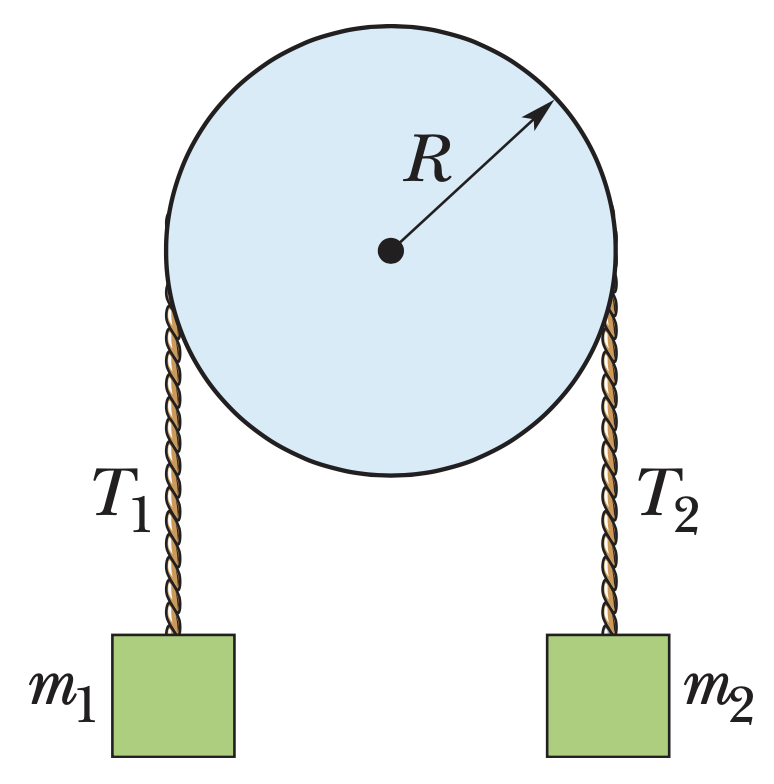
\includegraphics[scale=0.4]{Qfig13-4-20220425.png} 
  \caption{문제 4}
  \label{fig:4}
\end{figure}
\begin{itemize}
\item[(가)] 이 상자의 가속도의 크기는 얼마인가?
\item[(나)] 상자 1과 2에 걸리는 장력 $T_1$과 $T_2$를 구하여라.
\item[(다)] 이 도르래의 각가속도의 크기는 얼마인가?
  얼마인가?
\item[(라)] 도르래의 회전관성을 구하여라.
\end{itemize}

\noindent {\bf 풀이 : }
각 물체에 대한 자유 물체 다이어그램을 그리고 운동 방정식을 세워보자.
\begin{figure}[htp]
    \centering
    \begin{tikzpicture}
      \draw (-1.5,2.5) node {$m_1$ :} ;
      \draw (-2,0) -- (2,0) ;
      \draw (0,-2.5) -- (0,2.5) ;
      \draw [red,very thick,-latex] (0,0.1) -- (0,1.6) 
      node [left,black] {$T1$}; 
      \draw [blue,very thick,-latex] (0,-0.1) -- (0,-1.4) 
      node [left,black] {$m_1g$};
    \end{tikzpicture}
    \begin{tikzpicture}
      \draw (-1.5,2.5) node {$m_2$ :} ;
      \draw (-2,0) -- (2,0) ;
      \draw (0,-2.5) -- (0,2.5) ;
      \draw [red,very thick,-latex] (0,0.1) -- (0,1.8) 
      node [left,black] {$T_2$};
      \draw [blue,very thick,-latex] (0,-0.1) -- (0,-2.2) 
      node [left,black] {$m_2g$};
    \end{tikzpicture}
    \caption{자유 물체 다이어그램}
  \end{figure}
\begin{align}\label{eq:4-1}
    \begin{split}
        m_1:\sum F &= m_1a_1 = T_1 - m_1g,   \\
        m_2:\sum F &= m_2a_2 = m_2g - T_2.
    \end{split}
\end{align}
두 상자는 한 줄로 연결되어 있으므로,
\begin{align}\label{eq:4-2}
    a_1=a_2.
\end{align}
식 \eqref{eq:4-1}로 부터 각 상자의 가속도는 다음과 같다.
    \begin{align}\label{eq:4-3}
        a_1 = \frac{T_1-m_1g}{m_1},\,\,\,a_2 = \frac{m_2g-T_2}{m_2}
    \end{align}
\begin{itemize}
    \item[(가)] 
    상자 1은 이동거리가 $s=$ 75.0 cm, 걸린 시간 $t=$ 5.00 초, 
    초기 속력 $v_0=$ 0 m/s인 등가속도 운동을 하였으므로 다음과 같이 가속도를 구할 수 있다.
    \begin{align}\label{eq:4-4}
        s = \frac{1}{2}a_1t^2,\,\,\,a_1 = \frac{2s}{t^2}.
    \end{align}
    따라서 상자1 의 가속도 $a_1$은,
    \begin{align}
        \begin{split}
            a_1 &= \frac{2(75.0\,\mathrm{cm})}{(5.00\,\mathrm{s})^2} \\
            &= 6.00\,\mathrm{cm/s^2} = 6.00\times 10^{-2}\,\mathrm{m/s^2}.
        \end{split}
    \end{align}
    \item[(나)]
    식 \eqref{eq:4-1}으로 부터 다음과 같이 장력을 구할 수 있다.
    \begin{align}\label{eq:4-5}
       T_1 =m_1\left( a_1+g \right),\,\,\,
       T_2 =m_2\left( g-a_2 \right).
    \end{align}
    $m_1 = 460\,\mathrm{g}$이므로,
    \begin{align}
        \begin{split}
            T_1 &= (460\,\mathrm{g})
            ((6.00\times 10^{-2}\,\mathrm{m/s^2})+(9.80\,\mathrm{m/s^2})) \\
            &=(0.460\,\mathrm{kg})
            (9.86\,\mathrm{m/s^2}) \\
            &=4.54\,\mathrm{N}.
        \end{split}
    \end{align} 
    $m_2 = 500\,\mathrm{g}$이므로,
    \begin{align}
        \begin{split}
            T_2 &= (500\,\mathrm{g})
            ((9.80\,\mathrm{m/s^2})-(6.00\times 10^{-2}\,\mathrm{m/s^2})) \\
            &=(0.500\,\mathrm{kg})
            (9.74\,\mathrm{m/s^2}) \\
            &=4.87\,\mathrm{N}.
        \end{split}
    \end{align} 
    \item[(다)] 줄의 가속도를 $a$라고 하자. 
    줄이 미끄러지지 않으므로 도르래는 줄과 함께 회전하므로 도르래의 각가속도 $\alpha$는 
    다음과 같이 표현할 수 있다.
    \begin{align}\label{eq:4-6}
        \alpha=\frac{a_1}{R}.
    \end{align}
    따라서,
    \begin{align}
        \begin{split}
            \alpha&=\frac{(6.00\times 10^{-2}\,\mathrm{m/s^2})}
            {(5.00 \,\mathrm{cm})}
            = \frac{(6.00\times 10^{-2}\,\mathrm{m/s^2})}
            {(5.00\times 10^{-2} \,\mathrm{m})} \\
            &= 1.20\,\mathrm{rad/s^2}.
        \end{split}        
    \end{align}
    \item[(라)] 도르래에 감긴 줄에 작용하는 합력을 구하자. 자유 물체 다이어그램을 그려보면 다음과 같다.
    \begin{figure}[htp]
        \centering
        \begin{tikzpicture}
          \draw (-1.5,2.5) node {줄에 작용하는 합력 :} ;
          \draw (-3,0) -- (3,0) ;
          \draw (0,-1.5) -- (0,1.5) ;
          \draw [red,very thick,-latex] (0.1,0) -- (2.4,0) 
          node [above,black] {$T_2$};
          \draw [red,very thick,-latex] (-0.1,0) -- (-1.6,0) 
          node [above,black] {$T_1$};
        \end{tikzpicture}
        \caption{자유 물체 다이어그램}
    \end{figure}
    줄에 작용하는 합력 $T$는,
    \begin{align}\label{eq:4-7}
        T = T_2-T_1.
    \end{align}
    도르래에 작용하는 돌림힘 $\tau$은,
    \begin{align}
        \tau  = TR.
    \end{align}
    돌림힘과 각가속도를 알고 있으므로 도르래의 회전관성을 구할 수 있다. 도르래의 회전관성 $I$는,
    \begin{align}
        \tau = I\alpha,\,\,\, I=\frac{\tau}{\alpha}=\frac{TR}{\alpha}.
    \end{align}
    식 \eqref{eq:4-5}, \eqref{eq:4-6}과 식 \eqref{eq:4-7}로 부터,
    \begin{align}
        \begin{split}
            I &= \frac{(T_2-T_1)R^2}{a_1} =  \frac{(m_2\left( g-a_2 \right)
            -m_1\left( a_1+g \right))R^2}{a_1}  
            = \frac{((m_2-m_1)g-(m_2+m_1)a_1)R^2}{a_1} \\
            &=  \frac{(((500\,\mathrm{g})-(460\,\mathrm{g}))(9.80\,\mathrm{m/s^2})
            -((500\,\mathrm{g})+(460\,\mathrm{g}))
            (6.00\times 10^{-2}\,\mathrm{m/s^2}))(5.00\times 10^{-2}\,\mathrm{m})^2}
            {6.00\times 10^{-2}\,\mathrm{m/s^2}}    \\
            &= 13.9\,\mathrm{g\cdot m^2}=1.39\times 10^{-2}\,\mathrm{kg\cdot m^2}.
        \end{split}
    \end{align}
    도르래의 회전관성은 $1.39\times 10^{-2}\,\mathrm{kg\cdot m^2}$이다.
\end{itemize}


\vspace{1.cm}

\end{document}